\chapter{Das EVM8168-Entwicklungsboard}
\label{board}
\rm

F�r die in den folgenden Kapiteln beschriebenen Arbeitsschritte zur Portierung, Optimierung und Analyse des Programmes wurde ein EVM8168-Entwicklungsboard verwendet, welches von der Firma Texas Instruments in Zusammenarbeit mit der Firma Spectrum Digital entwickelt wurde.
Dieses Board kann mit Hilfe eines DM816x (DaVinci\texttrademark) ARM-Prozessors entweder selber Programme ausf�hren oder es k�nnen auch die beiden  ARM-Prozessoren C6A816x (Integra\texttrademark) oder AM389x (Sitara\texttrademark) emuliert werden. 
Da in dieser Arbeit der DaVinci\texttrademark-Prcessor verwendet wird, soll in Kapitel~\ref{sec:evm816} zun�chst das Board an sich und dann in Kapitel~\ref{sec:davinci} speziell der DaVinci\texttrademark betrachtet werden.

\section{Aufbau des EVM8168} \label{sec:evm816}
Wie in \cite{spec} beschrieben bietet das EVM8168-Entwicklungsboard eine Standalone-Plattform um Programme f�r DaVinci\texttrademark, Integra\texttrademark oder Sitara\texttrademark Prozessoren der Firma Texas Instruments zu entwickeln und debuggen. Hierf�r ist neben dem DaVinci\texttrademark noch weitere On-Board Perepherie auf dem Board aufgebracht. Unter anderem Anschl�sse f�r Gigabit Ethernet, VGA, HDMI und USB, sowie einen DSP.
F�r die in dieser Arbeit beschriebene Soundklassifikation wichtig sind au�erdem die Anschl�sse f�r  Line-In, Mic-In und Line-Out, sowie der integrierte AIC3106 Codec, welcher den eingehenden Soundstream f�r den DSP vorbereitet.
Abbildung~\ref{fig:top_ti816x_evm} zeigt eine Draufsicht auf das Entwicklungsboard und die unterhalb dessen angebrachte Daughtercard mit weiteren Anschlussm�glichkeiten.

\begin{figure}[htbp]
	\centering
		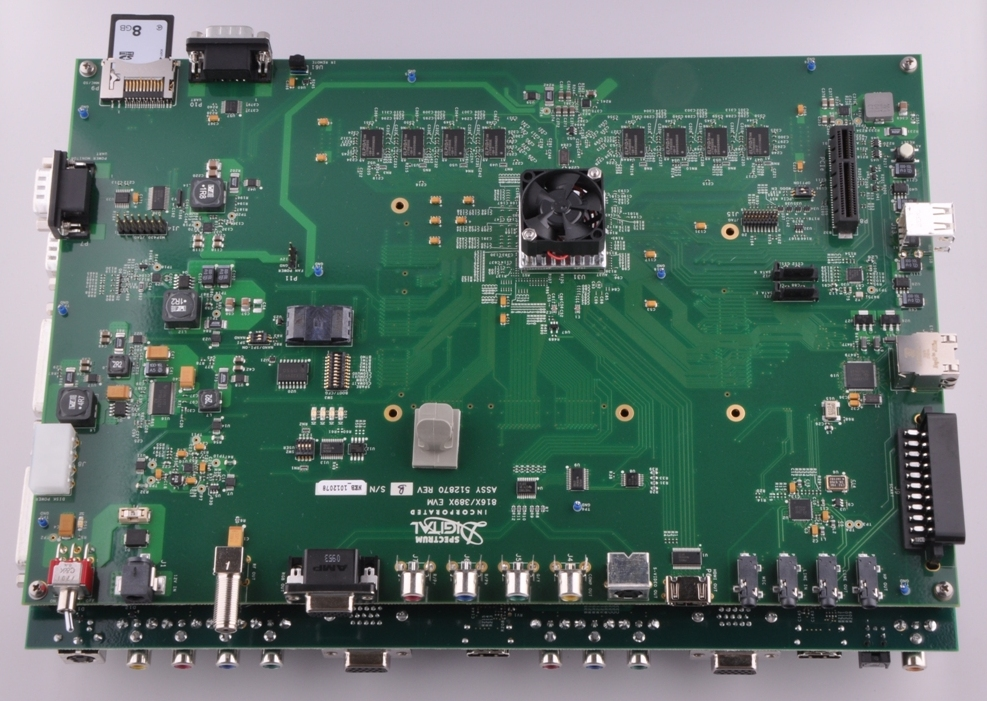
\includegraphics[scale=0.4]{../Pictures/top_ti816x_evm.png}
	\caption{Draufsicht auf das EVM8168}
	\label{fig:top_ti816x_evm}
\end{figure}



\section{Der DaVinci\texttrademark}\label{sec:davinci}